\documentclass{article}

\usepackage{ctex}
\usepackage{graphicx}
\graphicspath{{pic}}
\usepackage{amsmath}
\usepackage{siunitx}
\usepackage{amssymb}
%这两个包被用来输入商标R,TM符号和版权C符号。

\title{Week 3: git}
\author{Mayrain}
\date{\today}

\begin{document}

\maketitle

\section{Git}

\subsection{What is git}

\noindent
一个分布式的版本控制系统。分布式代表不需要联网,版本控制代表可以回溯文件修改历史。\\
有趣的部分:git是自托管的,也就是说git他自己的代码就是放在git仓库里的。现在你甚至可以在github上看到git的源代码。实现是用1000多行代码完成的。\\
git自带的git bash是一个命令行工具,可以用来操作git。他也很有用。\\

\subsection{How git works}

\noindent
\begin{align}
    working\quad directory & -> staging\quad area & ->  git  repository \notag \\
                           & add                  & commit \notag
\end{align}
他妈的这一段真丑啊我去,我得搞明白为什么排版会变成这样,但是不是现在。\\
push: 本地仓库 -> 远程仓库\\
pull: 远程仓库 -> 本地仓库\\
在这里课程讲的很简单,最好参见网络教程。\\
\\
利用git init folder可以新建一个文件夹并将其转化为git仓库。\\
git文件有三种状态:
\begin{itemize}
    \item untracked: 未跟踪
    \item modified: 已修改
    \item staged: 已暂存
    \item ignored: 已忽略
\end{itemize}
这里的ignored是指git不会跟踪这个文件,也就是说这个文件不会出现在git status的结果中。他被存储在gitignore文件。一般我们都在这里加一些规则。\\
github/gitignore: 这里有很多gitignore的规则,可以直接复制。\\
\\
commit message standards:\\
angular/angular:CONTRIBUTING.md\\
\\
作者的话:\\
老天,连git的commit的message都在github上有标准化的规定,不得不说这就是程序员的思维:机械而规范。让我想起了github上有名的“how to ask questions wisely”系列。很有意思。\\
\subsubsection{ADDITION:Commit Message Format}
*It is totally copy of angular/CONTRIBUTING.md.\\
\\
<header>\\
\\
Format: -> <Commit Type>(<Commit Scope>): <Short summary>\\
\\
Commit Type:\\
build: Changes that affect the build system or external dependencies (example scopes: gulp, broccoli, npm)\\
修改项目构建系统的代码或者外部依赖的改动,例如构建脚本,Dockerfile,package.json,webpack配置等等\\
ci: Changes to our CI configuration files and scripts (examples: CircleCi, SauceLabs)\\
修改项目继续集成流程的提交,例如Travis,Jenkins,GitLab CI,BrowserStack,SauceLabs等等\\
docs: Documentation only changes\\
仅仅修改了文档,比如README,CHANGELOG,CONTRIBUTE等等\\
feat: A new feature\\
新功能\\
fix: A bug fix\\
修复bug\\
perf: A code change that improves performance\\
提升性能的代码改动\\
refactor: A code change that neither fixes a bug nor adds a feature\\
代码重构\\
test: Adding missing tests or correcting existing tests\\
测试用例的变动\\
\\
Commit Scope:\\
indicate the place of the commit change.Should be the name of the npm package affected.Better to see this:\\
https://github.com/angular/angular/blob/main/CONTRIBUTING.md\\
\\
<Blank Line>\\
\\
<content>\\
\\
<Blank Line>\\
\\
<footer>\\
\\
\subsubsection{Version Name change rules}
version a.b.c[-d]\\
a: major version(主版本号,大改,不兼容的API修改。0表示开发阶段,不保证完整性)\\
b: minor version(次版本号,添加新功能,保持兼容)\\
c: patch version(修订号,兼容更改以及修正不正确的行为)\\
d: pre-release version(预发布版本号,代表这个程序是预发布的,实际上只是尝鲜版。顺序是alpha(内测), beta(公测), rc.1, rc.2, rc开头的都是预发布。)\\
\\
\subsection{Git Branch}
Branch,也就是分支,是相当于一个岔路指向标。在git中,我们可以创建分支,然后在分支上进行修改,最后将分支合并到主分支上。\\
如果我们在某个历史版本上做出一个修改,而不添加branch的话,那么当我们想要回到修改的版本时,就会发现我们的指针依然在master这个大branch上移动,而这个修改的版本,除非你记住了他的commit id,否则就无法回到这个版本了。(因为没有路标通向他,所以当到达分叉路口时系统会自动以为只有一条路,也就是master分支)\\
有两种创建分支的方法:\\
\begin{itemize}
    \item git branch <branch name>(基于当前的header,也就是分岔路口)
    \item git branch <branch name> <branch id>(基于当前所在分支的id提交,也就是根据这条路提交)
\end{itemize}
\section{github}
\noindent
GithubCLI是一个命令行程序,通过这个程序可以使用命令行操控github。\\
现在很多没能注意的就是,github的commit需要用签名去验证。在git中会出现一个verfied的图标,证明我使用我的私钥签名,并可以用公钥去验证。对比图如下:\\
\begin{figure}[h]
    \centering
    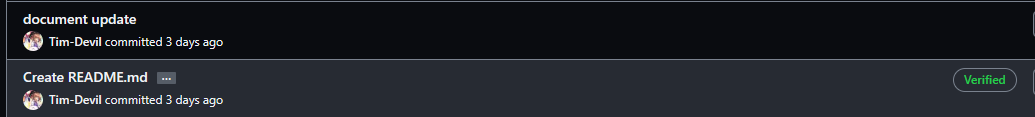
\includegraphics[width=\textwidth]{pic1_verfied.png}\\
\end{figure}
基于此我设置了github的公钥验证,在本地的git上打开了GPG签名。具体如何实现请详见b站tonycrane的录播。\\
\\
另外,github还给每个用户提供了二级域名,可以用仓库的组织形式去编写这一个域名作为自己的主页。对于每个仓库,他们也有自己的主页。\\
\\
github的action则是github提供的CI(持续集成)和CD(持续交付)工作。相当于配置自动化任务,在特定时间执行。\\
可以通过配置文件,文件名为.github/workflows/workflow\_name.yml。编写可以看见github官方文档。
\section{open-source software}
\subsection{oss versus free software?}
\noindent
所谓开源软件,意思就是公开源代码。将其源代码放在github上并设置repo为public就是开源。\\
自由软件则遵循四大原则:
\begin{itemize}
    \item 自由运行
    \item 自由修改
    \item 自由分发copy
    \item 自由分发modify
\end{itemize}
注意开源并不等效于完全自由。自由和开源完全不一样,即便是开源,也可以通过规定开源证书来约束用户如何使用源代码。\\
\\
copyright: 版权所有,一切权利归软件作者所有\\
书写方式:copyright\copyright 最初发表年-最初更新年 所有者. All rights reserved.\\
copyleft: 版权归作者所有,其他一切权利归任何人所有。他一定是自由软件。GPL就是一种copyleft许可证。
\subsection{license}
\subsubsection{No license?}
\noindent
没有许可证意味着:\\
原作者保留所有权利,不允许复制、分发、修改。如果需要使用,请联系原作者。(这个很反直觉,算是某种“最小权利”的约束吧。)
\subsubsection{Yes it has license!}
\noindent
\begin{figure}[h]
    \centering
    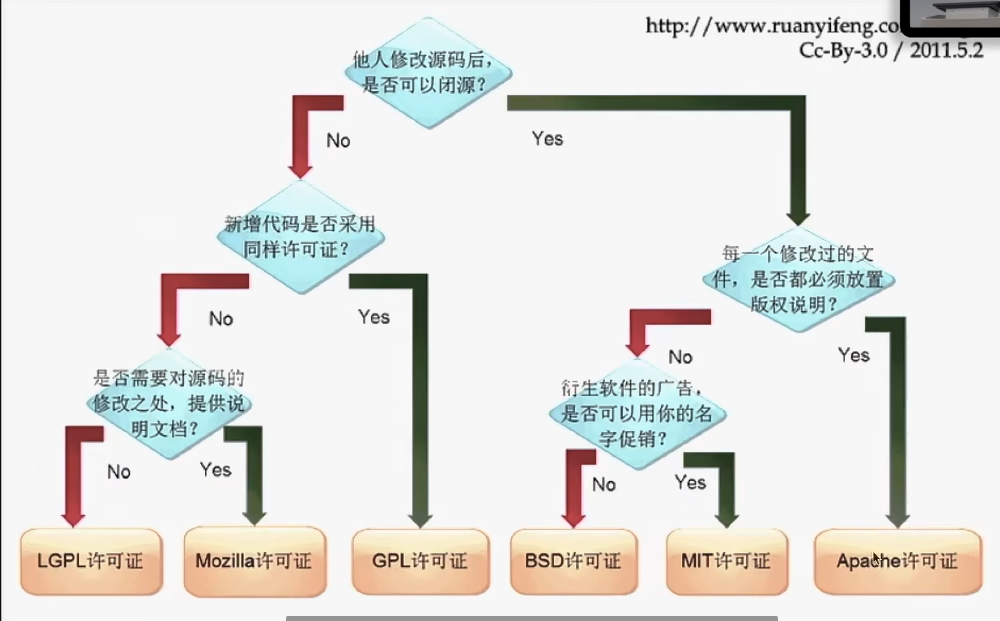
\includegraphics[width=0.9\textwidth]{pic2_license.png}
\end{figure}
也有一些变体,例如AGPL和LGPL
\subsubsection{Unlicense!}
\noindent
这个概念需要和没有许可证(我没有特意设置)的情况区分,unlicense意味着放弃所有权利,该软件进入公共领域。\\
\\
最后,详细的部分请见:\\
choosealicense.com
\subsection{How to use a license?}
\noindent
在根目录下包含文件LICENSE即可,其中附上许可证内容。github可以通过一些模板生成许可证,也会根据内容识别并显示许可证。\\
如果涉及多张许可证,都要放而且要声明许可证作用范围。\\
\subsection{License unrelevent with software}
\noindent
一些许可证并不是用于软件的……而是用于知识。例如cc(creative commons)许可证,用于知识共享。一般是用于知识型的内容,比如笔记。\\
详见:\\
creativecommons.org/share-your-work/cclicense/\\
官网上直接查看许可证内容,后缀改成txt就可以直接复制了。\\
注意github目前只识别cc 0(公共领域),cc by(需要标明原作者),cc by-sa(需要采用相同许可证)。
\section{github community}
\noindent
github的项目贡献,一般先看这些:
\begin{itemize}
    \item README
    \item CONTRIBUTING
    \item CODE\_OF\_CONDUCT
\end{itemize}
另外,提出issue之前,必须先查看是否有issue已经提出你的疑问!\\
And that's all. Thanks.
\end{document}